\section{Actividades con el repositorio GitHub}

\subsection{Creando e inicializando repositorio GitHub}
\begin{itemize}	
	\item Como ya tenemos nuestro repositorio GitHub y además esta clonado e inicializado en nuestra máquina local.
	\item Se realizaron los siguientes comandos en la computadora:
\end{itemize}	

\begin{lstlisting}[language=bash,caption={Creando carpeta de trabajo dentro de nuestro repositorio clonado en mi maquina local}][H]
	$ cd proyecto
   $ mkdir lab07
\end{lstlisting}
\begin{lstlisting}[language=bash,caption={Dirijíéndonos a la carpeta de trabajo}][H]
	$ cd lab07
\end{lstlisting}	
\begin{lstlisting}[language=bash,caption={Creando carpetas que contendrán el proyecto e imagenes}][H]
	$ cd lab07
   $ mkdir emailexample
   $ mkdir model_examples
   $ mkdir pdfs_examples
\end{lstlisting}

\subsection{Commits}
\begin{itemize}	
	\item A continucación se mostraran capturas de los commits, primero de la creacion de la carpeta de trabajo de lab07 y la carpeta de los ejemplos de envio de emails:
\end{itemize}	
\begin{figure}[H]
	\centering
	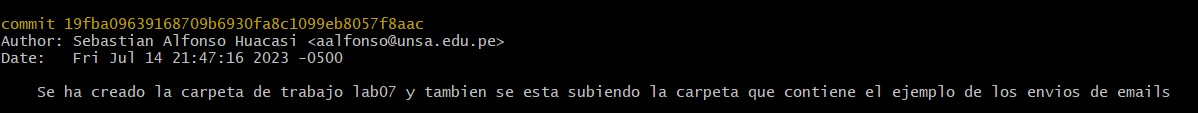
\includegraphics[width=0.8\textwidth,keepaspectratio]{img/1commit.jpg}
	%\includesvg{img/automata.svg}
	%\label{img:mot2}
	%\caption{Product backlog.}
\end{figure}
\begin{itemize}	
	\item Commit de la creacion de la carpeta de los ejemplos de model:
\end{itemize}
\begin{figure}[H]
	\centering
	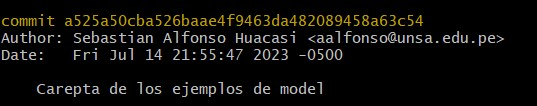
\includegraphics[width=0.8\textwidth,keepaspectratio]{img/2commit.jpg}
	%\includesvg{img/automata.svg}
	%\label{img:mot2}
	%\caption{Product backlog.}
\end{figure}
\begin{itemize}	
	\item Commit que indica que se estan subiendo la carpeta de los ejemplos de pdf y además los template:
\end{itemize}
\begin{figure}[H]
	\centering
	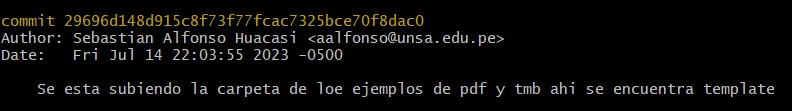
\includegraphics[width=0.8\textwidth,keepaspectratio]{img/3commit.jpg}
	%\includesvg{img/automata.svg}
	%\label{img:mot2}
	%\caption{Product backlog.}
\end{figure}
\begin{itemize}	
	\item Todo esto serían los archivos y orden de nuestro laboratorio 07:
\end{itemize}	
\begin{figure}[H]
	\centering
	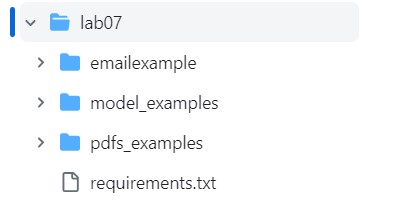
\includegraphics[width=0.8\textwidth,keepaspectratio]{img/estructura7.jpg}
	%\includesvg{img/automata.svg}
	%\label{img:mot2}
	%\caption{Product backlog.}
\end{figure}
\lstinputlisting[language=Python, caption={views.py-emails, se encuentra en la carpeta emailexample, dentro de la carpeta de send},numbers=left,]{src/views.py}
\begin{itemize}
        \item A continuación, procederé a explicar un poco el views.py de la parte de los emailsexample:
        \item from django.shortcuts import render: Importa la función render del módulo shortcuts de Django, que se utiliza para renderizar una plantilla y devolver una respuesta HTTP.
        \item from django.core.mail import send_mail: Importa la función send_mail del módulo mail de Django, que se utiliza para enviar correos electrónicos.
        \item def index(request): Define una función de vista llamada index que toma un objeto request como argumento. En Django, las funciones de vista se encargan de procesar las solicitudes HTTP y devolver respuestas.
        \item send_mail('Hola desde otra cuenta', 'Hello there. Esto es un mensaje automático.', 'sebastianalfonso2004@gmail.com', ['aalfonso@unsa.edu.pe'], fail_silently=False): Llama a la función send_mail para enviar un correo electrónico. Los parámetros proporcionados son:
        \item 'Hola desde otra cuenta': El asunto del correo electrónico.
        \item 'Hello there. Esto es un mensaje automático.': El cuerpo del correo electrónico.
        \item 'sebastianalfonso2004@gmail.com': La dirección de correo electrónico del remitente.
        \item ['aalfonso@unsa.edu.pe']: Una lista de direcciones de correo electrónico de los destinatarios.
        \item fail_silently=False: Indica que se debe generar una excepción si ocurre un error al enviar el correo electrónico.
        \item return render(request, 'send/index.html'): Renderiza la plantilla 'send/index.html' y devuelve la respuesta HTTP resultante. En este caso, la función de vista simplemente devuelve la plantilla sin modificar.
\end{itemize}
\lstinputlisting[language=Python, caption={views.py-pdfs, se encuentra en la carpeta pdfs_examples, dentro de la carpeta pdfs_example},numbers=left,]{src/viewss.py}
\begin{itemize}
        \item A continuación, procederé a explicar un poco el views.py de la parte de los pdfs_example:
        \item from django.http import HttpResponse: Importa la clase HttpResponse del módulo http de Django. HttpResponse se utiliza para devolver una respuesta HTTP desde una vista.
        \item from django.views.generic import View: Importa la clase View del módulo generic de Django. View es una clase base para vistas genéricas en Django.
        \item from django.template.loader import get_template: Importa la función get_template del módulo loader de Django. get_template se utiliza para cargar plantillas HTML.
        \item from .utils import render_to_pdf: Importa una función llamada render_to_pdf del módulo utils en el mismo directorio. Esta función se utiliza para generar un archivo PDF a partir de una plantilla HTML.
        \item def get(self, request, *args, **kwargs): Define un método get que manejará las solicitudes HTTP GET. Toma request y otros argumentos opcionales.
        \item template = get_template('pdf/invoice.html'): Carga la plantilla 'pdf/invoice.html' utilizando la función get_template.
        \item context = { ... }: Crea un diccionario context que contiene variables de contexto utilizadas en la plantilla. En este caso, incluye el número de factura, el nombre del cliente, el monto y la fecha actual.
        \item html = template.render(context): Renderea la plantilla con el contexto proporcionado, generando una cadena HTML.
        \item pdf = render_to_pdf('pdf/invoice.html', context): Genera un archivo PDF utilizando la función render_to_pdf y la plantilla junto con el contexto.
        \item response = HttpResponse(pdf, content_type='application/pdf'): Crea una instancia de HttpResponse con el contenido del archivo PDF y el tipo de contenido establecido como 'application/pdf'.
\end{itemize}
\subsection{Capturas de la ejecucion del laboratorio 07}
\begin{itemize}	
	\item Index email:
\end{itemize}	
\begin{figure}[H]
	\centering
	
\includegraphics[width=0.8\textwidth,keepaspectratio]{img/index.jpeg}
	%\includesvg{img/automata.svg}
	%\label{img:mot2}
	%\caption{Product backlog.}
\end{figure}
\begin{itemize}	
	\item Demostración del pdf:
\end{itemize}	
\begin{figure}[H]
	\centering
	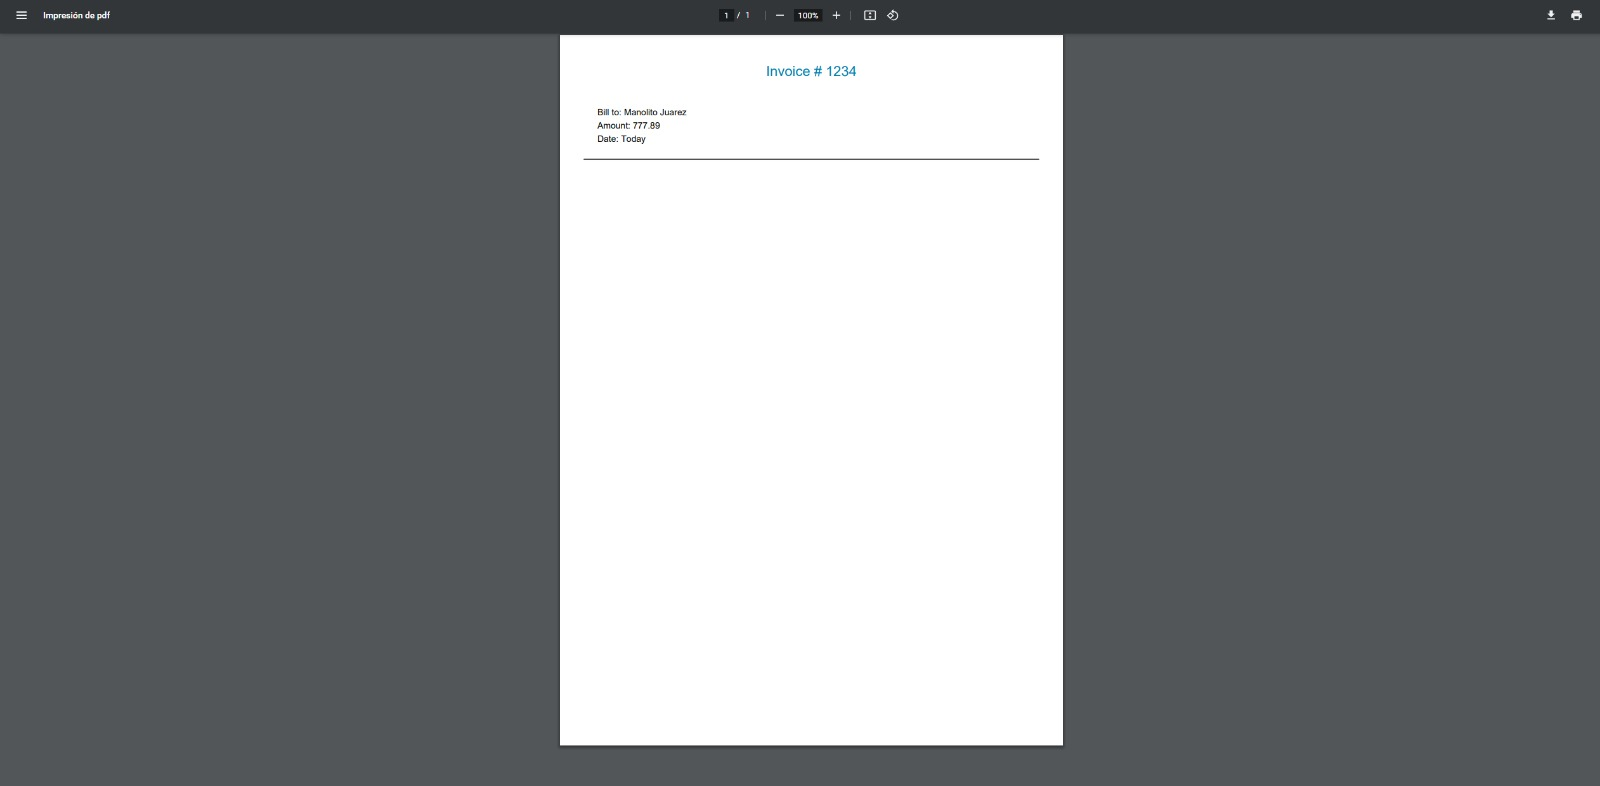
\includegraphics[width=0.8\textwidth,keepaspectratio]{img/pdf.jpeg}
	%\includesvg{img/automata.svg}
	%\label{img:mot2}
	%\caption{Product backlog.}
\end{figure}
\begin{itemize}	
	\item Email recibido, aumentandole algunas cosas más:
\end{itemize}	
\begin{figure}[H]
	\centering
	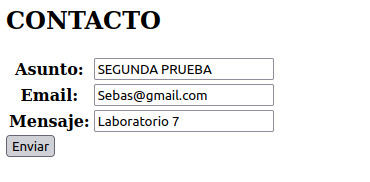
\includegraphics[width=0.8\textwidth,keepaspectratio]{img/e3.jpeg}
	%\includesvg{img/automata.svg}
	%\label{img:mot2}
	%\caption{Product backlog.}
\end{figure}
\begin{figure}[H]
	\centering
	
\includegraphics[width=0.8\textwidth,keepaspectratio]{img/e2.jpeg}
	%\includesvg{img/automata.svg}
	%\label{img:mot2}
	%\caption{Product backlog.}
\end{figure}
\begin{figure}[H]
	\centering
	
\includegraphics[width=0.8\textwidth,keepaspectratio]{img/e1.jpeg}
	%\includesvg{img/automata.svg}
	%\label{img:mot2}
	%\caption{Product backlog.}
\end{figure}
\begin{figure}[H]
	\centering
	
\includegraphics[width=0.8\textwidth,keepaspectratio]{img/e4.jpeg}
	%\includesvg{img/automata.svg}
	%\label{img:mot2}
	%\caption{Product backlog.}
\end{figure}
\subsection{Estructura de laboratorio 07}
\begin{itemize}	
	\item El contenido que se entrega del informe del laboratorio 07 es el siguiente:
\end{itemize}

\begin{lstlisting}[style=ascii-tree]
	Lab07-Informe/
   |--- informe-latex
	|--- contenido
   |   |--- actividades.tex
   |   |--- caratula.tex
   |   |--- github.tex
   |   |--- materiales.tex
   |   |--- preguntas.tex
   |   |--- referencia.tex
   |   |--- rubrica.tex
   |   |--- tarea.tex
	|--- img
   |   |--- logo_abet.png
   |   |--- logo_episunsa.png
   |   |--- logo_unsa.jpg
   |   |--- 1commit.jpg
   |   |--- 2commit.jpg
   |   |--- 3commit.jpg
   |   |--- e1.jpeg
   |   |--- e2.jpeg
   |   |--- e3.jpeg
   |   |--- e4.jpeg
   |   |--- estructura7.jpg
   |   |--- index.jpeg
   |   |--- pdf.jpeg
   |--- src
   |    |--- views.py
   |    |--- viewss.py
   |--- pweb2_lab07_aalfonso.pdf    
   |--- main.tex
\end{lstlisting}    